% Teaching content definitions.
% Use \DefineTeach{<number>}{...} where <number> matches the section numbering.
% Examples: 1, 1.2, 1.2.1

% 1) INTRODUCTION TO DATA SCIENCE
% 1.2 Tabular Data
%
% Use the structure below when adding teaching content.
% Note: \DefineTeach{1.2} is just an example to illustrate the format.
% \DefineTeach{1.2}{%
% % Write teaching content for "1.2 Tabular Data" here.
%
% % Template (copy and adapt):
% % \begin{examlikelihood}{Medium}
% % Why this appears on exams and how to recognize it.
% % \end{examlikelihood}
% %
% % \begin{examfavorite}
% % What instructors love to ask and typical phrasing.
% % \end{examfavorite}
% %
% % Why (motivation): ...
% % What (definition): ...
% % How (procedure/usage): ...
% %
% % \begin{cheatsheet}
% % \begin{itemize}
% %   \item Must‑memorize point 1
% %   \item Must‑memorize point 2
% % \end{itemize}
% % \end{cheatsheet}
% %
% % \begin{pitfall}
% % Common mistake and how to avoid it.
% % \end{pitfall}
% %
% % \begin{visualbox}
% % \centering
% % \begin{tikzpicture}[]
% % % Simple diagram
% % \end{tikzpicture}
% % \end{visualbox}
% %
% % \textbf{Key takeaways:} ...
% % }

% 1.4 Data Types
\DefineTeach{1.4}{%
\begin{visualbox}
\centering
\includegraphics[width=0.9\linewidth]{asset/data-types.png}
\end{visualbox}
}

% 1.5 Descriptive Statistics
\DefineTeach{1.5}{%
\begin{examlikelihood}{High}
Frequent: compute variance/STD/covariance/correlation by hand; read a correlation matrix.
\end{examlikelihood}

\begin{examfavorite}
Explain why covariance depends on units, and why correlation is normalized in $[-1,1]$.
\end{examfavorite}

Why (motivation): Quantify spread and association between variables.\\
What (definition): Variance/STD measure spread; covariance/correlation measure linear association.\\
How (procedure/usage): Compute formulas, then interpret sign/magnitude and check the correlation matrix.

\begin{cheatsheet}
\begin{itemize}
  \item \textbf{Variance (sample):} $s^2 = \frac{1}{n-1}\sum_{i=1}^{n}(x_i-\bar{x})^2$
  \item \textbf{Std dev:} $s = \sqrt{s^2}$
  \item \textbf{Covariance (sample):} $\mathrm{cov}(X,Y)=\frac{1}{n-1}\sum_{i=1}^{n}(x_i-\bar{x})(y_i-\bar{y})$
  \item \textbf{Correlation:} $r=\frac{\mathrm{cov}(X,Y)}{s_X s_Y}$ \; (unitless, $-1$ to $1$)
  \item \textbf{Correlation matrix:} table of pairwise correlations; symmetric with 1s on the diagonal.
\end{itemize}
\end{cheatsheet}

\begin{pitfall}
Correlation $\neq$ causation; a strong correlation can be driven by a confounder or Simpson's paradox.
\end{pitfall}

\begin{visualbox}
\centering
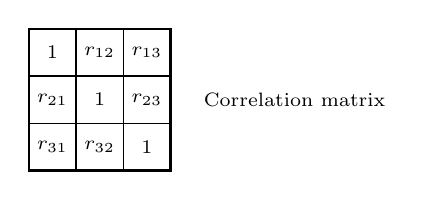
\begin{tikzpicture}[
  label/.style={font=\scriptsize},
]
% 3x3 correlation matrix sketch
\draw[thick] (0,0) rectangle (1.8,1.8);
\draw (0.6,0) -- (0.6,1.8);
\draw (1.2,0) -- (1.2,1.8);
\draw (0,0.6) -- (1.8,0.6);
\draw (0,1.2) -- (1.8,1.2);
\node[label] at (0.3,1.5) {1};
\node[label] at (0.9,1.5) {$r_{12}$};
\node[label] at (1.5,1.5) {$r_{13}$};
\node[label] at (0.3,0.9) {$r_{21}$};
\node[label] at (0.9,0.9) {1};
\node[label] at (1.5,0.9) {$r_{23}$};
\node[label] at (0.3,0.3) {$r_{31}$};
\node[label] at (0.9,0.3) {$r_{32}$};
\node[label] at (1.5,0.3) {1};
\node[label, right] at (2.1,0.9) {Correlation matrix};
\end{tikzpicture}
\end{visualbox}

\textbf{Key takeaways:} Know formulas + interpretations; correlation matrix is symmetric with 1s on the diagonal.
}

% 1.6 Basic Visualizations
\DefineTeach{1.6}{%
\begin{visualbox}
\centering
\includegraphics[width=0.9\linewidth]{asset/box-plot.png}
\end{visualbox}
}

% 1.7 Feature Transformations
\DefineTeach{1.7}{%
\begin{examlikelihood}{High}
Typical: pick the right transform (scale, log, encode) and explain why.
\end{examlikelihood}

\begin{examfavorite}
Identify data leakage in preprocessing; name the correct order for train/test transformations.
\end{examfavorite}

Why (motivation): Turn raw categorical/continuous variables into model-ready features.\\
What (definition): Encoding or discretizing features without changing the target meaning.\\
How (procedure/usage): Choose encoding by category type; choose binning by distribution.

\begin{cheatsheet}
\begin{itemize}
  \item \textbf{One-hot encoding:} create a 0/1 column per category (nominal).
  \item \textbf{Binary encoding:} represent categories as binary digits (compact one-hot).
  \item \textbf{Ordinal encoding:} map ordered categories to ranks (only if order is real).
  \item \textbf{Binning:} convert continuous to categories.
  \item \textbf{Equal-width binning:} fixed interval sizes across the range.
  \item \textbf{Equal-frequency binning:} same number of samples per bin.
\end{itemize}
\end{cheatsheet}

\begin{pitfall}
Fitting transforms on the full dataset (leakage). Always fit on training data, then apply to validation/test.
\end{pitfall}

\textbf{Key takeaways:} Use one-hot for nominal, ordinal for ordered labels, and binning for simplification.
}

% 2.1 Introduction to Decision Trees
\DefineTeach{2.1}{%
\begin{examlikelihood}{High}
Intro questions often ask you to explain how trees split data and what leaves represent.
\end{examlikelihood}

\begin{examfavorite}
Draw a small tree from a toy dataset or explain interpretability vs overfitting.
\end{examfavorite}

Why (motivation): Learn a function from labeled training instances to make predictions.\\
What (definition): A tree partitions the feature space by sequential if-then splits; leaves output a class or value.\\
How (procedure/usage): Choose splits to improve class purity or reduce prediction error.

\begin{cheatsheet}
\begin{itemize}
  \item \textbf{Goal:} learn a function $f(X)$ from labeled data to predict labels/values.
  \item \textbf{Tree structure:} root node, internal (non-leaf) nodes, leaf nodes.
  \item \textbf{Split rule:} one feature + threshold; paths are if-then rules.
  \item \textbf{Leaf meaning:} prediction (class/value) for that region of the space.
\end{itemize}
\end{cheatsheet}

\begin{pitfall}
Overly deep trees memorize training data; control with max depth, min samples, or pruning.
\end{pitfall}

\begin{visualbox}
\centering
\begin{tikzpicture}[
  node distance=8mm and 12mm,
  box/.style={draw, rounded corners, align=center, minimum width=26mm, minimum height=8mm},
  arrow/.style={-Latex, thick}
]
\node[box] (root) {$x_1 < 5?$};
\node[box, below left=of root] (l) {Leaf: Class A};
\node[box, below right=of root] (r) {$x_2 < 3?$};
\node[box, below left=of r] (rl) {Leaf: Class B};
\node[box, below right=of r] (rr) {Leaf: Class A};
\draw[arrow] (root) -- (l);
\draw[arrow] (root) -- (r);
\draw[arrow] (r) -- (rl);
\draw[arrow] (r) -- (rr);
\end{tikzpicture}
\end{visualbox}

\textbf{Key takeaways:} Trees learn $f$ from labeled data using splits; nodes/leaf roles are core.
}

% 2.2 Entropy and Information Gain
\DefineTeach{2.2}{%
\begin{examlikelihood}{Very High}
Almost guaranteed: compute entropy and information gain for candidate splits.
\end{examlikelihood}

\begin{examfavorite}
Given a small labeled dataset, compare splits and pick the one with highest information gain.
\end{examfavorite}

Why (motivation): Choose splits that make child nodes as pure as possible.\\
What (definition): Entropy measures impurity; information gain is impurity reduction.\\
How (procedure/usage): Compute parent entropy, child entropies, then IG = parent - weighted children.

\begin{cheatsheet}
\begin{itemize}
  \item \textbf{Entropy:} $H(S)=-\sum_{c} p_c \log_2 p_c$ (define $0\log 0 = 0$).
  \item \textbf{Weighted child entropy:} $\sum_{k}\frac{|S_k|}{|S|} H(S_k)$.
  \item \textbf{Information gain:} $\mathrm{IG}(S, \text{split})=H(S)-\sum_{k}\frac{|S_k|}{|S|} H(S_k)$.
  \item \textbf{Goal:} choose split with highest IG (most impurity reduction).
\end{itemize}
\end{cheatsheet}

\begin{pitfall}
Forgetting to weight child entropies by subset size; using raw entropy sums gives wrong IG.
\end{pitfall}

\begin{visualbox}
\centering
\includegraphics[width=0.75\linewidth]{asset/entropy-formula.png}
\vspace{2mm}
\includegraphics[width=0.75\linewidth]{asset/overall-entropy.png}
\vspace{2mm}
\includegraphics[width=0.75\linewidth]{asset/information-gain.png}
\end{visualbox}

\textbf{Key takeaways:} Compute entropy, weight children, pick split with highest IG.
}

% 2.3 ID3 Algorithm
\DefineTeach{2.3}{%
\begin{examlikelihood}{Very High}
Common: list the ID3 steps or run one iteration to choose the best split.
\end{examlikelihood}

\begin{examfavorite}
Explain stopping conditions and why ID3 prefers high information gain.
\end{examfavorite}

Why (motivation): Build a decision tree that best separates labeled data.\\
What (definition): ID3 is a greedy, top-down tree induction algorithm using information gain.\\
How (procedure/usage): Compute IG for each attribute, split on the best, and recurse.

\begin{cheatsheet}
\begin{itemize}
  \item \textbf{Input:} labeled dataset $S$ with categorical attributes (ID3 original).
  \item \textbf{Step 1:} if all labels same $\rightarrow$ make a leaf.
  \item \textbf{Step 2:} if no attributes left $\rightarrow$ leaf with majority class.
  \item \textbf{Step 3:} choose attribute with highest IG.
  \item \textbf{Step 4:} split $S$ by attribute values and recurse.
  \item \textbf{Output:} a decision tree; leaves store class label.
\end{itemize}
\end{cheatsheet}

\begin{pitfall}
ID3 favors attributes with many values; without corrections (e.g., gain ratio) it can overfit.
\end{pitfall}

\begin{visualbox}
\centering
\includegraphics[width=0.75\linewidth]{asset/id3-algo.png}
\vspace{2mm}
\includegraphics[width=0.75\linewidth]{asset/id3-example1.png}
\vspace{2mm}
\includegraphics[width=0.75\linewidth]{asset/id3-example2.png}
\end{visualbox}

\textbf{Key takeaways:} ID3 is greedy; compute IG, split, recurse, stop with pure/majority leaves.
}

% 2.4 Quantifying Information Gain
\DefineTeach{2.4}{%
\begin{examlikelihood}{Very High}
Often compute IG for a specific split and compare candidate attributes.
\end{examlikelihood}

\begin{examfavorite}
Show all intermediate steps: parent entropy, each child entropy, weighted sum, IG.
\end{examfavorite}

Why (motivation): Convert “best split” into a concrete, comparable number.\\
What (definition): IG = parent entropy minus weighted child entropies; Split Info measures how evenly the split divides data; Gain Ratio normalizes IG.\\
How (procedure/usage): Compute IG, then divide by split info to get gain ratio.

\begin{cheatsheet}
\begin{itemize}
  \item \textbf{Step 1:} compute parent entropy $H(S)$.
  \item \textbf{Step 2:} split by attribute values.
  \item \textbf{Step 3:} compute each child entropy $H(S_k)$.
  \item \textbf{Step 4:} compute weighted sum $\sum_k \frac{|S_k|}{|S|}H(S_k)$.
  \item \textbf{Step 5:} IG $= H(S) - \sum_k \frac{|S_k|}{|S|}H(S_k)$.
  \item \textbf{Split info (lecture: $H(d)$):} entropy of split proportions (how evenly data is partitioned).\\
  \hspace*{2mm}$H(d)=SI = -\sum_k \frac{|S_k|}{|S|}\log_2 \frac{|S_k|}{|S|}$.
  \item \textbf{Gain ratio:} $GR = \frac{IG}{H(d)}$ (same as $IG/SI$; penalizes many-valued attributes).
\end{itemize}
\end{cheatsheet}

\begin{pitfall}
Information gain is biased toward attributes with many values; use gain ratio to correct.
Also: weight by subset size and keep log base consistent.
\end{pitfall}

\begin{visualbox}
\centering
\includegraphics[width=0.75\linewidth]{asset/ig2-1.png}
\vspace{2mm}
\includegraphics[width=0.75\linewidth]{asset/igr-2.png}
\end{visualbox}

\textbf{Key takeaways:} IG is a weighted impurity reduction; higher is better.
}

% 2.5 Pruning
\DefineTeach{2.5}{%
\begin{examlikelihood}{High}
Often: explain why pruning reduces overfitting and name pre- vs post-pruning.
\end{examlikelihood}

\begin{examfavorite}
Given a tree, identify which branches to prune using validation error or complexity.
\end{examfavorite}

Why (motivation): Reduce overfitting by simplifying a deep tree.\\
What (definition): Pruning removes splits/branches that do not improve generalization.\\
How (procedure/usage): Stop early (pre-pruning) or cut back after training (post-pruning).

\begin{cheatsheet}
\begin{itemize}
  \item \textbf{Pre-pruning:} stop splitting early using rules like:
  max depth, min samples per node, min impurity decrease, min samples per leaf.
  \item \textbf{Post-pruning:} grow full tree, then prune using validation error or cost-complexity.
  \item \textbf{Goal:} simpler tree with similar or better validation performance.
\end{itemize}
\end{cheatsheet}

\begin{pitfall}
Pruning too aggressively can underfit; always tune on validation data, not test data.
\end{pitfall}

\begin{visualbox}
\centering
\includegraphics[width=0.75\linewidth]{asset/post-pruning.png}
\end{visualbox}

\textbf{Key takeaways:} Pruning trades depth for generalization; use validation to choose.
}
